\documentclass[a4paper,12pt,leqno]{article}
\usepackage[margin= 1 in]{geometry}
\usepackage[english]{babel}

\usepackage{amsmath}
\usepackage{amsfonts}
\usepackage{amssymb}
\usepackage{amsthm}
\usepackage{setspace}
\usepackage{natbib}
\bibliographystyle{plainnat}
\setlength{\bibsep}{0.0pt}
\setcitestyle{authoryear,open={(},close={)}}

\usepackage{multicol}
%\usepackage{indentfirst}
%\setlength{\parindent}{1}
\usepackage{booktabs}
\usepackage[labelfont=bf]{caption}
\usepackage{textgreek}
\usepackage{graphicx}
\usepackage{titlesec}


\setlength\parindent{0.25in}
\usepackage{indentfirst}
\graphicspath{ {./images/} }
\pagestyle{plain} 
\usepackage[T1]{fontenc}
\usepackage{mathptmx}
\usepackage{fixltx2e}
\usepackage[utf8]{inputenc}
\usepackage{libertine}
\usepackage{libertinust1math}
\usepackage{verbatim}
\usepackage{gb4e}

\title{\vspace{-0.6ex}Testing Tolerance Principle on Corpus Data}
\author{ }
\date{}
\begin{document}
%\noindent BUCLD 44 Proceedings\\
%To be published in 2020 by Cascadilla Press\\
%Rights forms signed by all authors\\

\maketitle



\vspace{1em}
%\begin{table}[htb]
\centering
\caption{Summary of corpus data}
\label{table:1}
\begin{tabular}{lllllll}
\toprule
 & \begin{tabular}[c]{@{}l@{}}Age of first recording to \\ first overregularizaiton error\end{tabular} & files & words & input words & verbs & input verbs \\
\toprule
Adam & 2;3 - 2;11 (\textit{feeled})& 18 & 39403 & 30366  & 6747 & 275 \\
Eve & 1;6 - 1;8 (\textit{seed})& 5 & 5304 & 11253  & 564 & 136\\
Sarah & 2;3 - 2;10 (\textit{topped})& 33 & 18778 & 27682 & 1759 & 293\\
Peter & 1;3 - 2;6 (\textit{broked})& 14 & 52769 & 95180 & 7532 & 633\\
Naomi & 1;3 - 1;11 (\textit{doed}) & 20 & 8009 & 9634 & 1240 & 222\\
Allison & 1;5 - 2;11 (\textit{throwed}) & 6 & 4605 & 9366 & 612 & 140\\
April & 1;10 - 2;1 (\textit{boughted}) & 2 & 1376 & 4435 & 128 & 100\\
Fraser & 2;0 - 2;5 (\textit{seed})& 90 & 137407 & 222200  & 13924 & 566 \\
\bottomrule
\bottomrule
Fraser_3 & & 3 & 1616 & 3304 & 1362 & 577 \\
Fraser_4 & & 4 & 1148 & 1495 & 1160 & 640\\
Fraser_5 & & 5 & 1485 & 1866 & 1339 & 757\\
Fraser_6 & & 6 & 1373 & 3206 & 1968 & 945\\
\bottomrule
\end{tabular}
\end{table}

\begin{table}[htb]
\centering
%\label{table:UEAB}
\caption{Number of observed total number of verb types, irregular verbs and exponents}
\begin{tabular}{lllllllll}
\toprule
 & $U_p$ & $\alpha_p$ & $U_c$ & $\alpha_c$ & $e_p$ & $\beta_p$ & $e_c$ & $\beta_c$ \\
\hline
Adam & 275 & 0.69 & 270 & 0.66 & 70 & 0.64 & 62 & 0.61 \\
Eve & 136 & 0.74 & 91 & 0.84 & 50 & 0.65 & 36 & 0.73 \\
Sarah & 293 & 0.71 & 189 & 0.77 & 68 & 0.58 & 48 & 0.62 \\
Peter & 633 & 0.64 & 424 & 0.69 & 83 & 0.51 & 67 & 0.54 \\
Naomi & 222 & 0.77 & 128 & 0.76 & 62 & 0.63 & 43 & 0.66 \\
Allison & 140 & 0.77 & 88 & 0.87 & 44 & 0.68 & 36 & 0.84 \\
April & 100 & 0.84 & 50 & 1.23 & 37 & 0.80 & 19 & 1.23 \\
Fraser & 566 & 0.56 & 358 & 0.60 & 97 & 0.44 & 78 & 0.49 \\
\bottomrule
\bottomrule
Fraser_3 & 155 & 0.80 & 84 & 0.85 & 54 & 0.64 & 38 & 0.70\\
Fraser_4 & 131 & 0.78 & 91 & 0.84 & 43 & 0.61 & 36 & 0.67\\
Fraser_5 & 145 & 0.79  & 95  & 0.8  & 53  & 0.63  & 33  &0.61\\
Fraser_6 & 179 & 0.76 & 135 & 0.85 & 57 & 0.6 & 39 & 0.71\\
\bottomrule
\end{tabular}
\end{table}

Insert all the numbers in table \ref{table:UEAB} to formulas below where ($U = N$):
\begin{exe}
\ex \label{newTN}Time complexity for a list of $N$ items without a productive rule ($T_N$):\\
$\begin{aligned}
T_N = & {\displaystyle\sum_{k=1}^N(r_i\cdot\frac{1}{r_i^\alpha\cdot H_{N,\alpha}})} = \frac{H_{N,\alpha-1}}{H_{N,\alpha}}
\end{aligned}$
\ex \label{newTR}Time complexity for a list with $e$ exceptions and a productive rule ($T_R$):\\
$\begin{aligned}
T_R = & \frac{H_{e,\beta-1}}{H_{e,\beta}}\cdot\frac{e}{N} + (1-\frac{e}{N})\cdot e
\end{aligned}$
\ex \label{newTP}A productive rule will be derived when $T_R \leq T_N$:\\
$\begin{aligned}
& \frac{H_{e,\beta-1}}{H_{e,\beta}}\cdot\frac{e}{N} + (1-\frac{e}{N})\cdot e & \leq  \frac{H_{N,\alpha-1}}{H_{N,\alpha}}
\end{aligned}$
\end{exe}
\begin{table}[htb]
\centering
\label{table:TRTNTR<TN}
\caption{Comparison between observed time complexity}
\begin{tabular}{llll|lll}
\toprule
 & \multicolumn{3}{l}{observed children's production} & \multicolumn{3}{l}{observed parents' input} \\
 \hline
 & $T_R$ & $T_N$ & $T_R \leq T_N$ & $T_R$ & $T_N$ & $T_R \leq T_N$ \\
Adam & 52.53 & 78.07 & True & 57.92 & 76.24 & True \\
Eve & 26.27 & 22.55 & \textbf{False} & 37.66 & 36.94 & \textbf{False} \\
Sarah & 39.94 & 47.90 & True & 57.62 & 78.67 & True \\
Peter & 60.18 & 115.04 & True & 76.05 & 181.99 & True \\
Naomi & 32.94 & 34.03 & True & 50.37 & 55.54 & True \\
Allison & 25.46 & 21.03 & \textbf{False} & 34.65 & 36.42 & True \\
April & 13.44 & 8.13 & \textbf{False} & 27.34 & 24.48 & \textbf{False} \\
Fraser & 67.27 & 110.64 & True & 86.71 & 181.58 & True\\
\bottomrule
\bottomrule
Fraser_3 & 26.36 & 20.75 & \textbf{False} & 41.38 & 38.27 & \textbf{False}\\
Fraser_4 & 26.52 & 22.55 & \textbf{False} & 33.77 & 33.82 & True\\
Fraser_5 & 25.61 & 24.69 & \textbf{False} & 40.08 & 36.56 & \textbf{False}\\
Fraser_6 & 31.33 & 31.41 & True & 45.03 & 46.24 & True\\
\bottomrule
\end{tabular}
\end{table}

\begin{table}[htb]
\centering

\caption{Mismatch between observed U and TP predicted N}
\label{table:MISMATCH}
\begin{tabular}{ccc}
\toprule
 & Observed $U$ & Expected $N$ \\
 \hline
Eve's production & 91 & ~120 \\
Eve's input & 136 & ~141 \\
Allison's production & 88 & ~117\\
April's production & 50 & ~152\\
April's input & 100 & ~111 \\
\bottomrule
\bottomrule
Fraser_3's production & 84 & ~94 \\
Fraser_3's input & 155 & ~176\\
Fraser_4's production & 91 & ~121 \\
Fraser_5's production & 95 & ~101\\
Fraser_5's input & 145 & ~169\\
\bottomrule
\end{tabular}
\end{table}

Table \ref{table:MISMATCH} showed that to produce a rule, expected N number of verb types need to be either produced by the child or learned from the parent. However, only observed U number of verb types have been found in corpus.  

\begin{exe}
\ex \label{eveagain}Minimum $N$ to confirm TP when $T_R$ = $T_N$:\\
$\begin{aligned}
& f(N) = T_R - T_N =
\frac{H_{e,\beta-1}}{H_{e,\beta}}\cdot\frac{e}{N} + (1-\frac{e}{N})\cdot e - \frac{H_{N,\alpha-1}}{H_{N,\alpha}} = 0
\end{aligned}$

\end{exe}
\begin{table}[!h]
\centering
\label{table:eoi}
\caption{Comparing the minimum \textit{N} and the observed \textit{U}}

\begin{tabular}{ccc|cc}
\toprule
 & Observed $U$ & Expected $N$ & Observed $e$ & Expected $e$\\
 \hline
Eve's production & 91 & ~120 & 36& ~28\\
Eve's input & 136 & ~141 & 50 & ~48 \\
Allison's production & 88 & ~117 & 36 & ~26 \\
April's production & 50 & ~152 & 19 & ~9\\
April's input & 100 & 111 & 37 &~31\\
\bottomrule
\end{tabular}
\end{table}
\section{Introduction}
\vspace{-1em}

\subsection{Deriving the Tolerance Principle}
\indent 

Rule-based learning, such as past-tense acquisition, is very commonly observed in language acquisition, as when children form the regular past tense for a novel verb in an experimental setting (\textit{wug} -> \textit{wugged}) (citation ?) or when they spontaneously produce an overregularization of an irregular verb (\textit{go} -> \textit{goed}) (citation). Such evidence indicates that the rule is productive since it outputs forms that the child has never encountered before. But what leads to use of rules in the first place? \citep{yang2016price} proposed the Tolerance Principle (TP) to predict when a productive rule will be deployed. He hypothesized that this happens when the cost of processing words is greater without using the rule than it is when using it. To estimate the cost, Yang based his calculations on three assumptions: 1) lexical retrieval, such as looking up the past tense of a verb in memory, is a self-terminating serial search process in which the order of search is based on word frequency; 2) a productive rule applies only after a search through exceptions to the rule; and 3) the distribution of children's effective vocabulary is Zipfian, that is, the product of a word's frequency times its frequency rank is a constant. Here we describe these assumptions in more detail and argue that the third assumption, that children's word frequency distributions are Zipfian, must be revised to account for child corpus data. We also demonstrate that corpus-based testing of the TP is sensitive to the density of the data in the corpus.

%Thus, he uses the TP to quantify a threshold number of exceptions ($\theta$) that a learner can tolerate: $\theta = N/ln(N)$.

Do children learn a rule for forming the past tense? Or do they simply have a list of verbs and local regularities? If they do have a rule, how is it formed, given that the input is noisy? \citep{yang2016price} has proposed the Tolerance Principle (TP) to explain how children deploy general (productive) rules given noisy input. We first describe the principle then our revision of it. Yang assumes that the humans apply the Elsewhere Condition  \cite[e.g.][]{mcclelland1981interactive, plaut1997structure} in processing rules and exceptions. The Elsewhere Condition can be implemented as a serial search procedure in which each lexical item is compared to all the exceptions to the general rule. If a match is found, a specific rule for the matching exception is triggered. If not, the general rule is applied as shown in (\ref{ewc}):
\begin{exe}
\ex \label{ewc}
\textsc{if} w = e_1 \textsc{then} apply rule e_1 to w... \\
\textsc{if} w = e_2 \textsc{then} apply rule e_2 to w...\\
\textsc{if} w = e_3 \textsc{then} apply rule e_3 to w...\\
...\\
\textsc{if} w = e_N \textsc{then} apply rule e_N to w...\\
\textsc{if} w not in set\{e_1,e_2,e_3,e_4....e_N\}, \textsc{then} apply general rule to w...
\end{exe}
For example, to retrieve the past tense form for the verb \textit{eat}, \textit{eat} is first compared to the exceptions in the irregular verb inventory. When it is found, the irregular rule for \textit{eat} is applied to derive the past tense form \textit{ate}. To retrieve the past tense form for the verb \textit{type}, when the search for a match in the irregular verb set fails, the general past tense rule is applied to derive \textit{typed}.

%MC: Assuming that lexical retrieval ...  ?
Since lexical retrieval is a self-terminating serial search process, rules and exceptions are organized to minimize the time required. A productive rule to produce a set of N items is derived when applying the rule takes less time than does processing all the items individually. Without a productive rule, all the items are ranked by their frequencies, so that frequently used items will be processed most quickly. When a productive rule is generated, items are separated into two categories, regulars and exceptions. The exceptions are ranked by frequency and the rule is applied only when the item is not found in the set of exceptions. For example, when there is no productive rule and the vocabulary inventory has \textit{n} regular items (\textit{w}) and \textit{m} irregular items (\textit{e}), all the items are arranged according to their frequency, as shown in (\ref{norule}). When there is a productive rule, all the irregular items are ranked based on frequency, and all the regular items are concatenated into a set where one rule will be applied, as shown in (\ref{rule}). 
\begin{exe}
\begin{minipage}{0.5\linewidth}
\ex Without productive rule:
\begin{equation*}
N = n+m \left\{\begin{array}{cc} 
 w_1 & frequency: 100 \\
 e_1 & frequency: 99\\
 w_2 & frequency: 98\\
 ... & frequency: ...\\
w_m & frequency: 2\\
e_n & frequency: 1
\end{array}
\right. \label{norule}
\end{equation*}
\end{minipage}
\begin{minipage}{0.5\linewidth}
\ex With productive rule:
\begin{equation*}
N = n+1 \left\{\begin{array}{cc} 
 e_1 & frequency: 99 \\
 e_2 & frequency: 90 \\
 e_3 & frequency: 87 \\
 ... & frequency: ...\\
 e_n & frequency: 1\\
 & {w_1,w_2,w_3...w_n} 
\end{array}
\right. \label{rule}
\end{equation*}
\end{minipage}
\end{exe}
The rule will be generated only when the cost (Yang refered to the cost as `time complexity') to process the list with the rule is less
than processing all the items. As shown in (\ref{norule}) and (\ref{rule}), there are fewer items (n+1) to process in the list with a productive rule than in the list without a productive rule (n+m). On occasion, however, the time to search for an item in the list \textit{with} a rule can be more than the search time in the list \textit{without} a rule. For example, for the item \textit{w_2}, which is a more frequent regular word, it will take less time to find \textit{w_2} in the list without a productive rule than in the list with one. Since \textit{w_2} is the third most frequent word, the search only needs to examine \textit{w_1} and \textit{e_1} before finding a match for \textit{w_2}. In the list with a productive rule, the regular item will be reached only after all the exceptions are checked, which creates more cost to find \textit{w_2}. Therefore, the rule will be deployed only when the average cost to search for each word in the list with a productive rule ($T_R$) is less than the list without a rule ($T_N$). 
\begin{exe}
\ex $T_{N} > T_{R}$
\end{exe}

According to Yang, the average cost to search for a word is the product of the probability of the word and the retrieval time for the word. To calculate the probability for each word, Yang assumes that any sample from a large corpus follows the Zipfian distribution; therefore, the product of the frequency of the word ($f_i$) and the rank ($r_i$) of the word is a constant ($C$).

\begin{exe}
\ex \label{Zipfian}
$r_if_i  = C_i$
\end{exe}
The probability of a word in a corpus ($p_i$) is the frequency of the word ($f_i$) divided by the sum of the frequencies of all the words. The probability of occurrence ($p_i$) for $w_i$ can be expressed as (\ref{p}) where $H_N = \displaystyle\sum_{k=1}^N \frac{1}{r_k}$.

\begin{exe}
\ex \label{p}
$\begin{aligned}
p_i &  = \frac{f_i}{\displaystyle\sum_{k=1}^N f_k} =\frac{\frac{C_i}{r_i}}{\displaystyle\sum_{k=1}^N \frac{C_k}{r_k}}=\frac{\frac{1}{r_i}}{\displaystyle\sum_{k=1}^N \frac{1}{r_k}}=\frac{1}{r_i\cdot H_N}&
\end{aligned}$
\end{exe}


Since all the items are stored in a list ranked according to frequency, the retrieval time for each item is determined by the rank of the item. For example, the word \textit{the} appears more frequently in the corpus than the word \textit{give}, and therefore it costs less to retrieve. Yang simplified this as `the \textit{i}-th ranked item takes \textit{i} units of time to be retrieved' \citep{yang2018user}. The cost for \textit{w_i} (T_{w_i}) is shown in (\ref{TW}). The total cost for \textit{N} items in the list ($T_N$) is shown in (\ref{TN}).
\begin{exe}
\ex \label{TW}
$\begin{aligned}
T_{w_i} & = r_i\cdot\frac{1}{r_i\cdot H_N} = \frac{1}{H_N}&
\end{aligned}$
\ex \label{TN}
$\begin{aligned}
T_N & = \displaystyle\sum_{k=i}^N (r_i\cdot\frac{1}{r_i\cdot H_N}) = \frac{N}{H_N}&
\end{aligned}$
\end{exe}

If a rule is used, all the exceptions are stored in a ranked list and all the regular items are stored in a set after the list of exceptions. The exception list is processed in the same way as is the list without rules. If there are \textit{e} items in the exceptions, the cost for \textit{e_i} (T_{e_i}) in the exception list is shown in (\ref{Tee}). The total cost for all the items in the exception list (T_e) is shown in (\ref{Tell}). 

%MC: these two formulas are incorrect and the explanation given in the preceding paragraph does not properly match
\begin{exe}
\ex \label{Tee}
$\begin{aligned}
T_{e_i} = r_i\cdot\frac{1}{r_i\cdot H_e}\cdot\frac{e}{N} = \frac{1}{N\cdot H_e}&
\end{aligned}$
\ex \label{Tell}
$\begin{aligned}
T_{e} = \displaystyle\sum_{k=1}^e(r_i\cdot\frac{1}{r_i\cdot H_e}\cdot\frac{e}{N}) = \frac{e}{H_e}\cdot\frac{e}{N}&
\end{aligned}$
\end{exe}

The cost for all regulars is the same, which is the constant $e$, given that there are $e$ items in the exception list. The total cost to process all the regular items (T_{\overline{w}}) is:
\begin{exe}
\ex \label{Tww}
$\begin{aligned}
T_{\overline{w}} =    (1 - \frac{e}{N})\cdot e
\end{aligned}$
\end{exe}
The total cost for a list with a productive rule ($T_R$) is the sum of the cost for exceptions and regular items, as shown in (\ref{Te}):
\begin{exe}
\ex \label{Te}
$\begin{aligned}
T_R = T_e + T_{\overline{w}} = & \frac{e}{N}\cdot \frac{e}{H_e} + (1-\frac{e}{N})\cdot e&
\end{aligned}$
\end{exe}
A productive rule will be derived only when $T_R$ is smaller than $T_N$. To derive the maximum number for the exceptions (\textit{e}), first we approximate the \textit{N}th harmonic number with the natural log (ln\textit{N}), then we make $T_R \leq T_N$:

\begin{exe}
\ex \label{TRR}
$\begin{aligned}
T_R &\leq T_N &\\
\frac{e}{N}\cdot \frac{e}{H_e} + (1-\frac{e}{N})\cdot e &\leq \frac{N}{H_N} &\\
\frac{e}{N}\cdot \frac{e}{lne} + (1-\frac{e}{N})\cdot e &\leq \frac{N}{lnN}\\
\frac{e^2}{N}\cdot (\frac{1}{lne} -1) + e & \leq \frac{N}{lnN}\\
\end{aligned}$
\end{exe}
Since $\frac{e^2}{N}\cdot(\frac{1}{lne} -1)$ is always smaller than or equal to zero, as long as $e$ is smaller than $\frac{N}{lnN}$,  then $T_R$ is always smaller than $T_N$. Thus, the TP is derived:
\begin{exe}
\ex \textit{Tolerance Principle} \label{TPTPT}\\
Let R be a rule applicable to \textit{N} items, of which \textit{e} are exceptions. \textit{R} is productive if and only iff:\\
$\begin{aligned}
&e \leq \theta_{N}, where \theta_{N} = \frac{N}{lnN}
\end{aligned}$ 
\citep[p.64]{yang2016price}
\end{exe}

\subsection{Why should(n't) the Tolerance Principle (TP) work?}
Recall that the TP assumes the Elsewhere Condition, and is derived based on the assumption that lexical retrieval is a serial search of a frequency-ranked list that results in the logarithmic relationship between frequency and retrieval time \citep{murray2004serial}. 
%MC: It's the serial search of a frequency-ranked list that results in the logarithmic relationship between frequency and retrieval time
%MC: In the following sentence, are you saying that it might not correspond to an actual psychological process? 
There is no guarantee that it corresponds to the actual psychological process learning. The TP appeaingly handles a critical fact about language acquisition: children generate rules based on noisy input. The TP provides an elegant and succinct way to quantify the `noise' in the input. 

Evidence from artificial language learning \citep{schuler2016testing} supports the TP. Children between the ages of 5 and 7 heard names of nine novel objects in both singular and plural forms. Each plural marker either followed a rule (add \textit{ka}) or instead used an individual suffix (add \textit{po, tay,  lee bae, muy,} or \textit{woo}). In one condition, children heard five nouns with the \textit{ka} marker and four with individual markers. In another condition, they heard three nouns with the \textit{ka} marker and six with individual markers. As the TP predicts, children learned the rule under the 5/4 condition but not the 3/6 condition, as shown by their ability to use \textit{ka} as a general plural marker in a Wug-like test. 

Despite this evidence, other research has queried whether the TP can be applied to explain language acquisition in real life. 

Yang used $lnN$ as the approximation of the Harmonic number, as shown in (\ref{TRR}). For smaller $N$, however, {$\log_2 N$} is a better approximation of $H_N$ \citep{andreae2018charles}. For example, in \cite{schuler2016testing}'s experiment, when N = 9, $H_9 \approx 2.83$, while $\ln 9 \approx 2.20$ and $\log_2 9 \approx 2.71$. For N = 9, the base-2 logarithm is a better approximation than the natural logarithm. That the values matter can be seen by looking at the 4 exceptions, which were calculated based on $\theta =  N/lnN$, where 9/2.20 $\approx 4.10$. If, instead, the original $H_9 \approx 2.83$ were inserted, then $\theta =  N/H_N$ would be 9/2.83 $\approx 3.18$. That result produces a tolerance threshold of three exceptions, which goes against the results in \cite{schuler2016testing}.  

The TP also received criticism on the more general level of how to approach acquisition. For example, perhaps communicative needs, context, prior learning and cognitive load should be taken into account \citep{goldberg2018sufficiency}. As another example, serial search might be a flawed model compared to a more relevant lexical retrieval model \citep{kapatsinski2018intolerance}\footnote{See \cite{yang2018some} for his response to Goldberg and Kapatsinski.}.
%MC: for Yang's defense of serial search??

In addition, Yang examined Adam's and Eve's corpus data on past tense verbs to test the TP. However, the results didn't conform to TP predictions. There are more irregular verbs in Adam's and Eve's data than the maximum number of exceptions ($\theta$) the TP predicts. Yang attributed the discrepancy to sampling effects. 


In this paper, we developed a method to test the TP on corpus data and explored how would sampling effects influence the applicability of the TP on the corpus data. The rest of the paper is organized as follow: in section 2, we revisited Yang's test on Adam and Eve and proposed a revised methods that would be more appropriate for corpus data testing; in section 3, we tested the revised method on eight children's corpus data, including Adam and Eve; in section 4, we used Fraser's corpus (a densely sampled corpus from Manchester corpus) to explore the sampling effects on the TP. 


\section{Revised Testing Methods}
\subsection{Yang's Test on Adam's and Eve's Data}
In Chapter 4 of \cite{yang2016price}'s book, he established a procedure for the applying the TP. In our study, we followed his procedure. 
\begin{exe}
\ex 
\begin{xlist}
\ex Obtain a rule \textit{R} along with its structural description and structural change. 
\ex Count \textit{N}, the number of lexical items that meet the structural description of \textit{R}.
\ex Count \textit{e}, the subset of \textit{N} that are exceptions to R.
\ex Compare \textit{e} and the critical threshold $\theta_N = \frac{N}{lnN}$ to determine productivity.
\end{xlist}
\end{exe}

Yang applied this procedure to explain the acquisition of past tense in English children. English speaking children usually start to produce the past-tense form by the age of 2. Most children also produce overregularization errors on past tense, such as \textit{grewed}, \textit{feeled} \citep[e.g.][]{marcus1992overregularization}. The first instance of an overregularization error can be seen as an unambiguous marker for the presence of a productive `add \textit{-d}' rule for past tense. 

Adam produced his first overregularization error at the age of 2;11, when he said \textit{What dat feeled like?} \citep{brown19731}. This error implied that Adam had already constructed the past tense rule.  
According to the TP's prediction, the number of irregular verbs that Adam knew (\textit{e}) must be smaller than $\theta = N/lnN$, where $N$ is the number of all the verbs in his vocabulary. Adam's first recording starts at 2;3. Yang thus estimated Adam's effective vocabulary (\textit{N}) as all the verbs he produced between 2;3 and 2;11. Yang did not only count all the past tense verbs, he counted all forms of verbs as $N$. According to Yang, as long as Adam produced one form of a verb, that verb has to be in Adam's lexicon. Based on this method, he found 300 verbs, which made \textit{N} = 300. Therefore, $\theta = N/lnN \approx 53$, which means Adam can learn the rule when there are fewer than 53 irregular verbs. However, Yang counted 57 irregular verbs in Adam's total 300 verb lexicon. He attributed the difference between 57 and 53 to sampling effects. 

Yang used the same method to test Eve's data. Eve's first overregularization error appeared at 1;10 when she said \textit{it falled in the briefcase}\footnote{Yang made an error here. Eve made the first overregularization error at the age of 1;8, when she said \textit{I seed it}.} \citep{brown19731}. Yang found 163 verbs Eve produced between the age 1;6, when Eve had her first recording, and 1;10. When $N = 163$, $\theta = N/lnN \approx 32$, which means Eve could only tolerate 32 irregular verbs in order to produce the past tense rule. However, Yang found 49 irregulars in her production, which is again higher than what the TP predicts. He attributed the difference to undersampling of Eve's data.  

\subsection{Revised Testing Methodology}
In Yang's test, the TP failed to account for Adam's and Eve's corpus data on past tense acquisition. With the proposed new methodology, we aim to preserve Yang's insight of the TP, which is that a rule will be derived if the cost to retrieve an item from a list with a rule is smaller than from a list without a rule. We develop a different version of the TP and altered the formula to calculate the cost to retrieve an item. 

First, we aim to better estimate the probability of each item ($p_i$) in a list or items ranked by frequency. Yang assumed a Zipfian distribution for all items $N$ and all the exceptions $e$. However, a Zipfian distribution is not guaranteed for a small corpus, such as all the verbs and irregular verbs a 2-year-old child knows, which affects how $p_i$ is derived. Yang's formula for $p_i$ (\ref{CCC}) is based on a convenient fact of Zipfian distribution: when a corpus follows a Zipfian distribution, the product of the frequency of a word ($f_i$) and the rank of that word ($r_i$) is a constant $C$,shown in (\ref{AAA}). This is derived from the formal expression of Zifp's law, which is shown in (\ref{powerlaw}): the frequency of the $r$th most frequent word is inversely proportional to its rank, where the exponent ($\alpha$) equals 1. Formula (\ref{AAA}) is only valid when $\alpha$ is 1, when $N$ has a Zifpian distribution. When a smaller corpus (such as children's effective vocabulary of verbs and irregular verbs) has a power law distribution but doesn't necessarily a Zifpian distribution, where the exponent ($\alpha$) is not 1, formula (\ref{Zipfian}) is no longer valid, thus $p_i$ needs to be recalculated. 
\begin{exe}
\ex 
\begin{xlist}
\ex \label{AAA}
$\begin{aligned}
r_i \cdot f_i = C
\end{aligned}$ (replicate of (\ref{Zipfian}))
\ex \label{CCC}
$\begin{aligned}
p_i &  = \frac{f_i}{\displaystyle\sum_{k=1}^N f_k} =\frac{\frac{C_i}{r_i}}{\displaystyle\sum_{k=1}^N \frac{C_k}{r_k}}=\frac{\frac{1}{r_i}}{\displaystyle\sum_{k=1}^N \frac{1}{r_k}}=\frac{1}{r_i\cdot H_N}&
\end{aligned}$ (replicate of (\ref{p})
\end{xlist}
\ex \label{powerlaw}
$\begin{aligned}
f_i = Cr_i^{-\alpha}, \alpha = 1
\end{aligned}$
\end{exe}
In this paper, we propose to measure the actual corpus distributions of all the verbs ($N$) and the irregular verbs ($e$), and use the empirically estimated exponents that best fit those ranked frequency distributions in our calculations. Since all the verbs and all the irregular verbs do not necessarily share the same distribution, we will use $\alpha$ and $\beta$ to represent the exponents for these two distributions respectively. To include the exponent as a variable, the probability formula can be written as follow, where $H_{n,m} = \displaystyle\sum_{k=1}^n \frac{1}{k^m}$:
\begin{exe} 
\ex \label{newp}Probability of occurrence for $i$th ranked word ($p_i$):\\
$\begin{aligned}
p_i = & \frac{\frac{1}{r_i^\alpha}}{\displaystyle\sum_{k=1}^N (\frac{1}{r_k^\alpha})} = \frac{1}{r_i^\alpha\cdot H_{N,\alpha}}
\end{aligned}$ 
\end{exe}
Based on the new formula for $p_i$, the cost to retrieve an item from a list without rules ($T_N$) and the cost to retrieve an item from a list with rules ($T_e$) can be written as follow:
\begin{exe}
\ex \label{newTN}Cost for a list of $N$ items without a productive rule ($T_N$):\\
$\begin{aligned}
T_N = &{\displaystyle\sum_{k_1}^N(r_i\cdot p_i)}\\
= & {\displaystyle\sum_{k=1}^N(r_i\cdot\frac{1}{r_i^\alpha\cdot H_{N,\alpha}})} \\
= & \frac{H_{N,\alpha-1}}{H_{N,\alpha}}
\end{aligned}$
\ex \label{newTR}Cost for a list with $e$ exceptions and a productive rule ($T_R$):\\
$\begin{aligned}
T_R = &{\displaystyle\sum_{k_1}^e (r_i\cdot p_i)} \cdot \frac{e}{N} + (1-\frac{e}{N}) \cdot e\\
= & \frac{H_{e,\beta-1}}{H_{e,\beta}}\cdot\frac{e}{N} + (1-\frac{e}{N})\cdot e
\end{aligned}$
\ex \label{newTP}A productive rule will be derived when $T_R \leq T_N$:\\
$\begin{aligned}
& \frac{H_{e,\beta-1}}{H_{e,\beta}}\cdot\frac{e}{N} + (1-\frac{e}{N})\cdot e & \leq  \frac{H_{N,\alpha-1}}{H_{N,\alpha}}
\end{aligned}$
\end{exe}

Unlike formula (\ref{TRR}) where $H_N$ can be conveniently approximated using $lnN$, there is no mathematical approximation for the Harmonic number in the inequation (\ref{newTP}). Therefore, the new version of the TP is not going to produce a maximum number of the irregular items; instead, we propose to compare $T_R$ and $T_N$ directly. The Tolerance Principle will be confirmed if $T_R$ is smaller than $T_N$ as predicted in (\ref{newTP}). 

In the next section, we extracted all the variables ($e$, $N$, $\alpha$ and $\beta$) from eight children's corpora to compare $T_N$ and $T_R$. Instead of counting all the verb types the child produced as the $N$, we also estimate the $N$ by using the verb types from parents input. Since $N$ represents the child's effective vocabulary, children's production and parents' input represent the lower and upper boundary of the vocabulary respectively. The type of irregular verbs $e$ is counted as long as one form of the irregular verb (not necessarily the past tense form) appear in children's production or parents' input. The distribution of $N$ and $e$ are then mapped to the best fitted power law function to calculate the exponent $\alpha$ and $\beta$. 
\section{Testing the TP on corpus data}

\textbf{Use Yang's original TP to test}
\subsection{Testing on Adam's, Eve's and six other children's corpus data}
In this section, we use the revised testing methods to test eight children's corpus data on their past tense acquisition. The age of the first recording and the age of the first overregularization error for each child is shown in \textsc{table} \ref{table:1}, with a summary of the each child's corpus data.

\begin{table}[htb]
\small
\centering
\caption{Summary of corpus data for each child}
\label{table:1}
\begin{tabular}{llllllll}
\toprule
 & \begin{tabular}[c]{@{}l@{}}Age of first recording to \\ overregularizaiton error\end{tabular} & corpus & files & words & \begin{tabular}[c]{@{}l@{}}input\\words \end{tabular} & verbs & \begin{tabular}[c]{@{}l@{}}input\\words \end{tabular} \\
\toprule
Adam(\textit{feeled}) & 2;3 - 2;11 & \cite{brown19731}&18 & 39403 & 30366  & 6747 & 4670 \\
Eve & 1;6 - 1;8 (\textit{seed})& \cite{brown19731} &5 &  5304 & 11253  & 564 & 1618\\
Sarah & 2;3 - 2;10 (\textit{heared}) &\cite{brown19731}&33  & 18778 & 27682 & 1759 & 3867\\
Peter & 1;3 - 2;6 (\textit{broked})& \cite{bloom1974imitation}& 14 &52769 & 95180 & 7532 & 15537\\
Naomi & 1;3 - 1;11 (\textit{doed}) & \cite{sachs1983talking} &20  &8009 & 9634 & 1240 & 1463\\
Allison & 1;5 - 2;11 (\textit{throwed}) & \cite{bloom1973one} &6 &  4605 & 9366 & 612 & 1453\\
April & 1;10 - 2;1 (\textit{boughted}) & \cite{higginson1985fixing}& 2 & 1376 & 4435 & 128 & 658\\
Fraser & 2;0 - 2;5 (\textit{seed})& \cite{lieven2009two} &90 &  137407 & 222200  & 13924 & 32359 \\
\bottomrule
\end{tabular}
\end{table}
All of the data were automatically extracted from the annotated corpora in CHILDES using the \textsc{nltk} python package. The verbs in each file were identified using part-of-speech taggers annotated by the MOR program \citep{macwhinney2012morphosyntactic}. The number of verb types and irregular verb types in parents' input ($U_p$ and $e_p$) and in children's production ($U_c$ and $e_c$) are shown in \textsc{table} \ref{table:UEAB}, with the exponents for the verb types of parents' input ($\alpha_p$), children's production ($\alpha_c$) and the exponents for the irregular verb types in parents' input ($\beta_p$) and the children's production ($\beta_c$). The log-log graphs for each child can be found in the Appendix.


\begin{table}[htb]
\centering
\caption{Number of observed total number of verb types, irregular verbs and exponents}
\label{table:UEAB}
\begin{tabular}{lllllllll}
\toprule
 & $U_p$ & $\alpha_p$ & $U_c$ & $\alpha_c$ & $e_p$ & $\beta_p$ & $e_c$ & $\beta_c$ \\
\hline
Adam & 275 & 0.69 & 270 & 0.66 & 70 & 0.64 & 62 & 0.61 \\
Eve & 136 & 0.74 & 91 & 0.84 & 50 & 0.65 & 36 & 0.73 \\
Sarah & 293 & 0.71 & 189 & 0.77 & 68 & 0.58 & 48 & 0.62 \\
Peter & 633 & 0.64 & 424 & 0.69 & 83 & 0.51 & 67 & 0.54 \\
Naomi & 222 & 0.77 & 128 & 0.76 & 62 & 0.63 & 43 & 0.66 \\
Allison & 140 & 0.77 & 88 & 0.87 & 44 & 0.68 & 36 & 0.84 \\
April & 100 & 0.84 & 50 & 1.23 & 37 & 0.80 & 19 & 1.23 \\
Fraser & 566 & 0.56 & 358 & 0.60 & 97 & 0.44 & 78 & 0.49 \\
\bottomrule
\end{tabular}
\end{table}

First, we used Yang's method ($\theta = N/lnN$) to calculated the theoretical threshold for learning and compared it with the observed number of irregular verbs. The results in shown in \textsc{table} \ref{yang1}. We used $U_c$ and $U_p$ to represent $N$ separately and inserted the value of the variables ($e$, $\alpha$, $\beta$) to formula (\ref{newTN}) and (\ref{newTR}) to calculate $T_N$ and $T_R$. The results for $T_R$ and $T_N$ for each child is shown in \textsc{table} \ref{table:TRTNTR<TN}. 







\begin{table}[htb]
\centering
\caption{Comparison between observed cost and the TP predicted cost}
\label{table:TRTNTR<TN}
\begin{tabular}{cccc|ccc}
\toprule
 & \multicolumn{3}{l}{$N$ = Children's production ($U_c$)} & \multicolumn{3}{l}{$N$ = Parent's input ($U_p$)} \\
 \hline
 & $T_R$ & $T_N$ & $T_R \leq T_N$ & $T_R$ & $T_N$ & $T_R \leq T_N$ \\
Adam & 52.53 & 78.07 & True & 57.92 & 76.24 & True \\
Eve & 26.27 & 22.55 & \textbf{False} & 37.66 & 36.94 & \textbf{False} \\
Sarah & 39.94 & 47.90 & True & 57.62 & 78.67 & True \\
Peter & 60.18 & 115.04 & True & 76.05 & 181.99 & True \\
Naomi & 32.94 & 34.03 & True & 50.37 & 55.54 & True \\
Allison & 25.46 & 21.03 & \textbf{False} & 34.65 & 36.42 & True \\
April & 13.44 & 8.13 & \textbf{False} & 27.34 & 24.48 & \textbf{False} \\
Fraser & 67.27 & 110.64 & True & 86.71 & 181.58 & True\\
\bottomrule
\end{tabular}
\end{table}

As shown in \textsc{table} \ref{table:TRTNTR<TN}, the TP successfully predicted five children's acquisition on past tense acquisition, that the past tense rule is derived because $T_R$ is smaller than $T_N$. However, three children's data (Eve, Allison and April) do not support the TP's prediction. This could be attributed to the effect of smaller sample size, since Eve, Allison and April have less data between the first recording and the first appearance of the overregularization error than other children (as shown in \textsc{table} \ref{table:1}). In order to further test how would sample size affect the testablibity of the TP, we used Fraser's corpus to explore the sampling effects on the TP.  


\subsection{Exploring Small Sample effects on the TP}
Fraser is the most densely sampled corpus in this study. His first recording and first overregularization error was 5 month apart and he had 90 recording files. He was recorded for five hours per week in the first month (2;0 to 2;1) and one hour per week for the rest of the four months (2;2 to 2;5). The densely sampled corpus captured 358 types of verbs and 78 types of irregular verbs that Fraser produced, and 566 types of verbs and 97 types of irregular verbs in parents' input. Eve's, April's and Allison's corpus are less densely sampled comparing to Fraser's. Eve's first recording and first overregularization error was only 2 month apart and she only had 5 recording files. She was recorded twice a month between the age of 1;6 - 1;8. April's first recording and first overregularization error was 3 months apart and she was only recorded twice (1;10 and 2;1). Allison's first recording and first overregularizaiton error was 18 months apart and she was recorded only six times. Four of her 6 files were recorded before 2;0 (1;5, 1;7, 1;8 and 1;10) and only 2 files were recorded after she turned two years old (2;4 and 2;10). The short intervals between the age of overregularization error and the first recording (such as Eve and April) could be the reason for a smaller sample since the children simply didn't produce enough verbs in such short time intervals. Or, the smaller sample could be a result of sparse sampled data (such as Alison) that the recordings failed to cover the children's longitudinal development. In this section, we used Fraser's corpus to explore these two types of small sample. 

We first investigated the age related small sample size effect by setting the age of first recording as 2;4, only one month before Fraser made the first overregularization error (2;5). There are 11 recording files between 2;4 - 2;5 in Fraser's corpus, and a summary of the corpus data is shown in \textsc{table} \ref{table:FraserSum}. Then, we randomly selected 3,4,5,6 files from Fraser's corpus to represent different density of the corpus from age 2;0 - 2;5. The summary of the corpus is also shown in \textsc{table} \ref{table:FraserSum}. Subsequently, the number of verb types and irregular verb types in children's production ($U_c$ and $e_c$) and parents' input ($U_p$ and $e_p$), and the exponent for the distribution of all verbs ($\alpha_c$ and $\alpha_p$) and irregular verbs  ($\beta_c$ and $\beta_p$) are subtracted from the data, shown in \textsc{table} \ref{table:FraserB}. These variables were then inserted into formula (\ref{newTN}) and (\ref{newTR}) to calculate the $T_N$ and $T_R$. The results are shown in \textsc{table} \ref{table:Fraser<}.

\begin{table}[htb]
\centering
\caption{Summary of Corpus used Small Sample Effects testing}
\label{table:FraserSum}
\begin{tabular}{llllllll}
\hline
& & Age & files & words & input words & verbs & input verbs \\
\toprule
Age Related & Fraser_{age} & 2;4 - 2;5 & 11 & 2861 & 4074& 2104&5497\\
\hline 
Density Related & Fraser_3 & 2;3, 2;4, 2;5 & 3 & 1616 & 3304 & 1362 & 577 \\
& Fraser_4 & 2;0, 2;1,2;3, 2;4 & 4 & 1148 & 1495 & 1160 & 640\\
& Fraser_5 & 2;0x3, 2;1, 2;2 & 5 & 1485 & 1866 & 1339 & 757\\
& Fraser_6 & 2;0x3, 2;1, 2;2, 2;4& 6 & 1373 & 3206 & 1968 & 945\\
\bottomrule
\end{tabular}
\end{table}

\begin{table}[htb]
\centering
\caption{Number of observed total number of verb types, irregular verbs and exponents in Fraser's samples}
\label{table:FraserB}

\begin{tabular}{llllllllll}
\toprule
& & $U_p$ & $\alpha_p$ & $U_c$ & $\alpha_c$ & $e_p$ & $\beta_p$ & $e_c$ & $\beta_c$ \\
\hline
Age Related & Fraser_{age} & 277 & 0.66& 168& 0.73&71& 0.53& 54&0.60\\
\hline
Density Related &Fraser_3 & 155 & 0.80 & 84 & 0.85 & 54 & 0.64 & 38 & 0.70\\
&Fraser_4 & 131 & 0.78 & 91 & 0.84 & 43 & 0.61 & 36 & 0.67\\
&Fraser_5 & 145 & 0.79  & 95  & 0.8  & 53  & 0.63  & 33  &0.61\\
&Fraser_6 & 179 & 0.76 & 135 & 0.85 & 57 & 0.6 & 39 & 0.71\\
\bottomrule
\end{tabular}
\end{table}

\begin{table}[!ht]
\centering
\caption{Comparison between the cost in Fraser's samples}
\label{table:Fraser<}
\begin{tabular}{lllll|lll}
\toprule
& & \multicolumn{3}{l}{$N$ = Children's production ($U_c$)} & \multicolumn{3}{l}{$N$ = Parent's input ($U_p$)} \\
\hline
& & $T_R$ & $T_N$ & $T_R \leq T_N$ & $T_R$ & $T_N$ & $T_R \leq T_N$ \\
 \hline
Age Related & Fraser_{age} & 42.58 & 45.48 &True & 59.31& 79.99 & True\\
\hline
Dense Related & Fraser_3 & 26.36 & 20.75 & \textbf{False} & 41.38 & 38.27 & \textbf{False}\\
&Fraser_4 & 26.52 & 22.55 & \textbf{False} & 33.77 & 33.82 & True\\
&Fraser_5 & 25.61 & 24.69 & \textbf{False} & 40.08 & 36.56 & \textbf{False}\\
&Fraser_6 & 31.33 & 31.41 & True & 45.03 & 46.24 & True\\
\bottomrule
\end{tabular}
\end{table}

As shown in \textsc{table} \ref{table:Fraser<}, the TP was tested to be true using only one month of Fraser's data. It implies that the short time interval between the first recording and the overregularization error does not affect the testability of the TP. However, the density of the sample has a more substantial impact on whether the TP can be tested. For Fraser's data, the TP was successfully tested on six files, but not three to five files, as shown in \textsc{table} \ref{table:Fraser<}. 
\section{Discussion}
In language acquisition, rule-based learning is very common, such as past-tense acquisition. But what leads to rule learning in the first place? Yang proposed the Tolerance Principle predict when a rule will be productive. He hypothesizes when the cost to process a word in a list with a rule is minimum a rule will be produced. In order to estimate the cost to process a word, he based his calculations on two assumptions: 1) lexical retrieval is a serial search process; 2) the distribution of children's effective vocabulary is Zipfian. Thus, he uses the TP to quantify a threshold number of exceptions ($\theta$) that a learner can tolerate: $\theta = N/ln(N)$. However, the corpus data doesn't support the threshold predicted by the TP. Yang examined Adam's and Eve's data and neither conform to the TP's threshold. 

This paper revisted his second assumption in the TP calculation and revised the testing methodology to make it more appropriate for the corpus data. We then used the revised methods to test eight children's past-tense acquisition data (including Adam's and Eve's). Five of the  eight children's data support the TP's prediction. We further investigated the other three children's data and explored how sample size affects the testability of the TP. The results showed that the TP requires a relatively densely sampled corpus to be tested true. 

What is a "densely sampled corpus"? Based on our empirical data, $N$ needs to be at least over 120 and the $e$ has to be less than 33\% of $N$. However, we don't have any good explanation. The density of the corpus could affect all four variables in the TP formula, the number of types of items $N$ and exceptions $e$, and the distribution of $N$ and $e$, thus changing the exponent $\alpha$ and $\beta$. The interaction of the four variables and their relationship to the TP worth further investigation.  
\newpage
\section*{Appendix}
\begin{figure}[!htb]
\begin{minipage}{0.48\linewidth}
    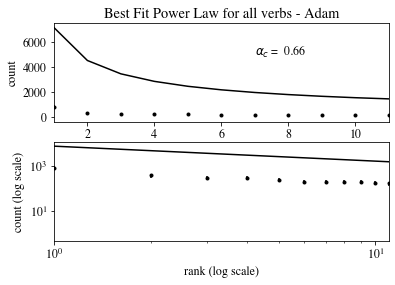
\includegraphics[scale=0.4]{AAC.png}
    \caption{Distribution of Adam's Verbs}
\end{minipage}
\begin{minipage}{0.54\linewidth}
    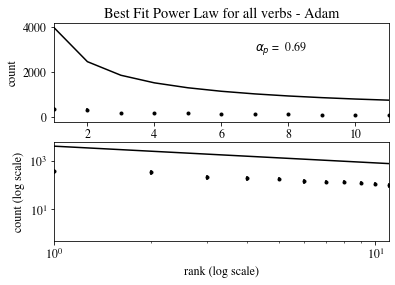
\includegraphics[scale=0.4]{AAP.png}
    \caption{Distribution of Adam's mother's verbs}
\end{minipage}
\end{figure}
\vspace{-2em}
\begin{figure}[!htb]
\begin{minipage}{0.48\linewidth}
\centering
    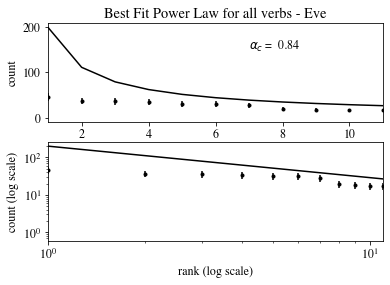
\includegraphics[scale=0.4]{EAC.png}
    \caption{Distribution of Eve's Verbs}
\end{minipage}
\begin{minipage}{0.53\linewidth}
\centering    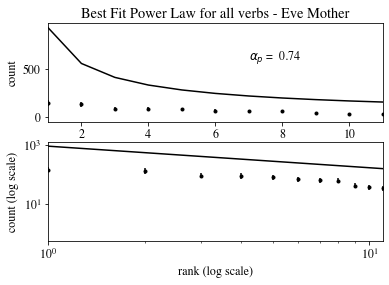
\includegraphics[scale=0.4]{EAP.png}
    \caption{Distribution of Eve's mother's verbs}
\end{minipage}
\end{figure}
\vspace{-2em}
\begin{figure}[!htb]
\begin{minipage}{0.5\linewidth}
    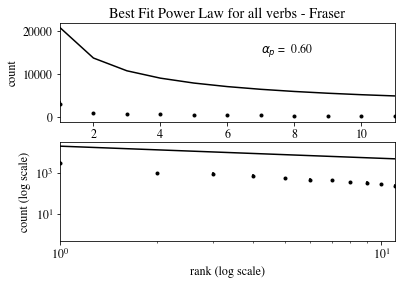
\includegraphics[scale=0.4]{FAC.png}
    \caption{Distribution of Fraser's Verbs}
\end{minipage}
\begin{minipage}{0.55\linewidth}
    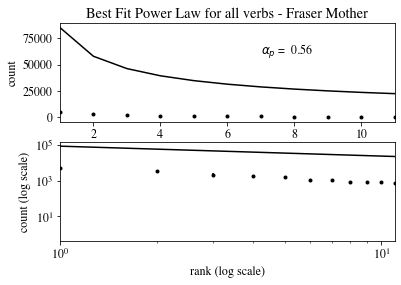
\includegraphics[scale=0.4]{FAP.png}
    \caption{Distribution of Fraser's mother's verbs}
\end{minipage}
\end{figure}
\vspace{-2em}
\begin{figure}[!htb]
\begin{minipage}{0.5\linewidth}
    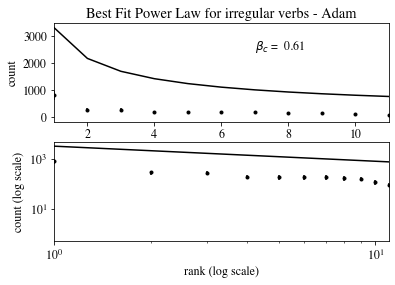
\includegraphics[scale=0.4]{ABC.png}
    \caption{Distribution of Adam's Irregular Verbs}
\end{minipage}
\begin{minipage}{0.5\linewidth}
\centering    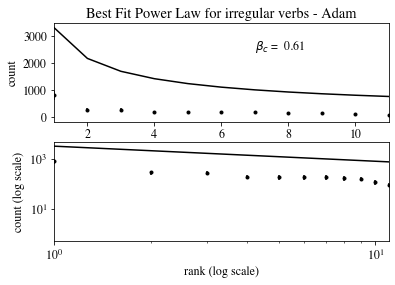
\includegraphics[scale=0.4]{ABC.png}
    \caption{Distribution of Ada's mother's Irregular verbs}
\end{minipage}
\end{figure}
\vspace{-2em}
\begin{figure}[!htb]
\begin{minipage}{0.5\linewidth}
    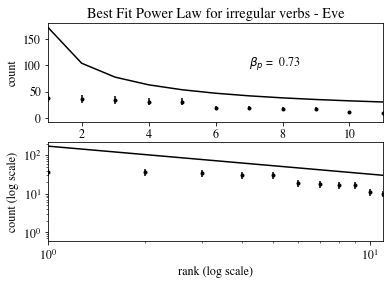
\includegraphics[scale=0.4]{EBC.png}
    \caption{Distribution of Eve's Irregular Verbs}
\end{minipage}
\begin{minipage}{0.5\linewidth}    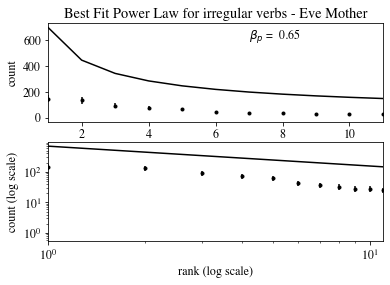
\includegraphics[scale=0.4]{EBP.png}
    \caption{Distribution of Eve's mother's Irregular verbs}
\end{minipage}
\end{figure}
\vspace{-2em}
\begin{figure}[!htp]
\begin{minipage}{0.5\linewidth}
    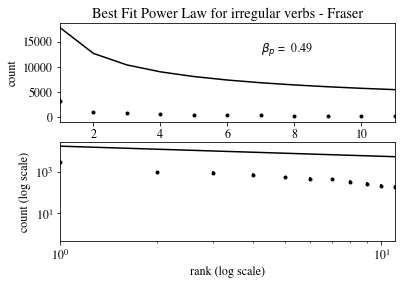
\includegraphics[scale=0.4]{FBC.png}
    \caption{Distribution of Fraser's Irregular Verbs}
\end{minipage}
\begin{minipage}{0.5\linewidth}
    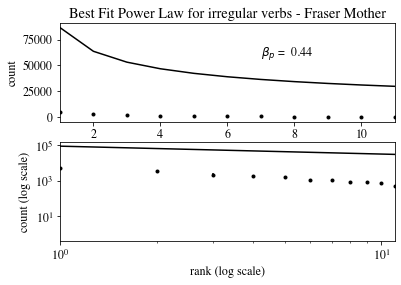
\includegraphics[scale=0.4]{FBP.png}
    \caption{Distribution of Fraser's mother's Irregular verbs}
\end{minipage}
\end{figure}
\clearpage
\bibliography{bib}
\end{document}

